%%
%% Indiana University Dissertation Template
%%
%% This is a LaTeX template for a dissertation that adheres to the 
%% guidelines of the Indiana University Graduate School.
%%
%% It is mosly based on a template circulated by the Mathematics 
%% Department. Some examples of how to structure and organize the 
%% directories in a way that suits dissertations using additional figures
%% have been added.
%%
%% Required files: 
%% - MasterFile[Dissertation].tex (this file, the main file that loads all
%%		all relevant files)
%% - iuphd.cls (this file contains the definitions for basic global formatting. 
%%		There is probably no reason to touch this file, but if you are having
%%		trouble with the formatting, title page (or anything before the 
%%		first chapter), appendices, etc., you might fix it here.)
%% - dissertationBibliography.bib (the file that contains all of the references 
%%		cited in the dissertation. You could divide the references into 
%%		individual .bib files according to chapter, but this could cause
%%		problems with references that occur in multiple chapters)
%% - dissertationStyle.sty (this file takes the place of what would normally
%%		appear in the preamble of a shorter document. If you need to 
%%		modify or add any packages, do so here.)


\documentclass[showabstract,showacknowledgments,showdedication]{iuphd} 

\usepackage{dissertationStyle}

% For title and abstract page

\title{My Very Important Study}
\author{Author McAuthorson}
\date{November 2019} % Completion date of Dissertation
\department{Linguistics} % Change this to your department

% For acceptance and abstract page

\committeechair{Kenneth de Jong, PhD}
\readertwo{Julie Auger, PhD}
\readerthree{Stuart Davis, PhD}
\readerfour{Sharlene Newman, PhD}
\readerfive{Dennis Preston, PhD}
\defensedate{September 20, 2019} % Date of PhD defense

% For Copyright Page
\cryear{Year} % Copyright year

\begin{document}
\maketitle
\acceptancepage

% This page is optional
%\copyrightpage


% This page is optional but generally included

\begin{acknowledgments}


Here's where where you acknowledge people and institutions.
You can write whatever you want, but it's somewhat standard to thank people in groups from most professional (your advisers, colleagues, research groups) to most personal (your friends and family). 
Funding sources are almost always listed at the end.

 

\end{acknowledgments}

% This page is optional

\begin{dedication}
For those who are about to rock\\
We salute you
\end{dedication}

% This page is optional

%\begin{preface}
%This is the (optional) preface page which can be used if you wish. This page should appear after the dedication (or acknowledgements page if there is no dedication page) and before the abstract page.
%\end{preface}

% % This page is required

\begin{abstract}
Here is where your abstract goes.
The graduate school doesn't specify a strict page limit, but 250--300 words is typical.

According to the Graduate School: ``As many people will learn about your work through your abstract published in the ProQuest Dissertations \& Theses Database, you should spend a good bit of effort in the composition of both the abstract and the title of your work. Try to convey the flavor of your work, not just the bare bones of your findings. You should also work to phrase your title so that it truly describes the contents and will be easily found in the index of the database. The index is based on key words, so be as specific as you can be about your subject.''

\newpage

\end{abstract}



% This page is required

\tableofcontents

\chapter{Introduction}

Here is the introduction.
It's where you talk about your study and how cool it is.
If you want to cite someone, you can do it like this \cite{preston1999}.
Of course, if you want to cite \citeA{preston1986}, you'd do it like this.
Check out the APAcite documentation if you need to cite things in another way.

\section{A new section}

In this section, I'll insert a figure. 
Figure \ref{fig:koala} shows a koala in the rain.

\begin{figure}[b!]
\centering
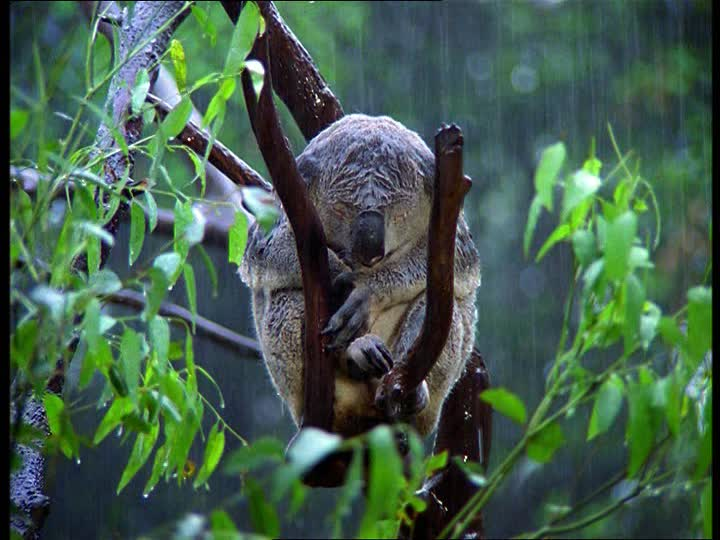
\includegraphics[width=1\textwidth]{koala}
\caption{This is a koala in the rain}
\label{fig:koala}
\end{figure}

To paraphrase Ze Frank, this koala evidences an abundance of apathy regarding its situation.

\subsection{A subsection}

Sometimes it is useful to have two images as part of the same figure.
Figure \ref{fig:unlikelyEvents} shows a cat (briefly) being sweet to a dog and a location that Kramer refers to as the ``nexus of the universe.''

\begin{figure}[ht!]
\centering
\subfloat[]{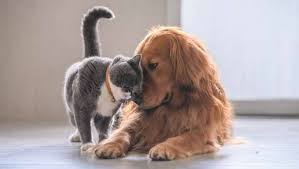
\includegraphics[width=0.45\textwidth]{dogAndCat}}
\subfloat[]{
\includegraphics[width=0.45\textwidth]{nexusOfUniverse}}
\caption{Examples of inauspicious events.}
\label{fig:unlikelyEvents}
\end{figure}	

\chapter{Methods}

Here are the methods.

\chapter{Analysis}

Here is the analysis.

\chapter{Conclusion}

Here is the conclusion.


\newpage

% \appendix command is necessary to change chapter numbering.
% Appendices are optional

\appendix

\chapter{Word List and Reading Passages}

Below are the word list and reading passages read by the participants in the state-wide study.

\section{Rainbow Passage}

Rainbow Passage (contains a mixture of oral and nasal consonants in the approximate proportion found in everyday speech)
When the sunlight strikes raindrops in the air they act like a prism and form a rainbow. The rainbow is a division of white light into many beautiful colors. These take the shape of a long round arch with its path high above and its two ends apparently beyond the horizon. There is according to legend a boiling pot of gold at one end. When a man looks for something beyond his reach, his friends say he is looking for a pot of gold at the end of the rainbow. 
\vspace{11pt}

\noindent Citation for rainbow passage: Fairbanks, G. (1960). Voice and articulation drillbook, 2nd edn. New York: Harper \& Row. (pp. 124-139).


\section{Mike's Party}

Mike was planning to throw a party on Tuesday night, and decided to check his list one more time before he went shopping. He already had plenty of stuff to drink, and he had enough plates and cups. His brother Jim was going to bring some fish he'd caught and maybe put them on the grill. Mike thought he should get some chips, pretzels, and a few other snacks to start the meal. He looked around to see if he had anything sweet, but then remembered that his friend Linda was baking a cake. When he looked in the cupboard, he saw that he was out of coffee. He found a pencil, wrote it down on his list, and hoped it was on sale. Then he went to the garage, got in his car, and went to the 7-11. It looked like everything would go well.
\vspace{11pt}

\noindent This passage was developed by Dennis Preston and Jon Bakos to target Midland and Southern features


\section{A Bad Day for Ducks}

Tom and Bob were supposed to meet at Tom's house. They planned to got to a nearby pond and watch the ducks. While waiting for Bob to get there, Tom picked up around the house. He put the electric fan away for the winter and did the dishes.

He wanted a snack before he left , so he peeled an apple and cut it into slices. He bit into one, but it was awful, probably rotten. He spit it out and tried to rinse his mouth out with hot black coffee. He poured it into a tin cup, but when he put it up to his lips he spilled it on his hand. His hand puffed up and hurt a lot, so he stuck it under the faucet to make it feel better.

He grabbed a dusty hat out of the closet and shook it, but he couldn't get the dirt off. He got a cap instead and put a scarf around his neck and put on his socks and boots. There was a big hole in his sock, and Bob was really late. It was already past 2:00. Nothing was working out.

Just then Bob phoned and said he wanted to talk. He told Tom that the flock of ducks had left the pond. A pack of dogs had chased them off. Tom was sad; he had really wanted to see the ducks, but Bob said that they could go shoot some pool instead. Tom thought that was a good idea and forgot all about the ducks and his burned hand.

\vspace{11pt}

\noindent This passage was developed by Dennis Preston and students to target Northern Cities features.


\section{Wordlist}

These wordlist items were selected to include key dialect features of the Inland North, Northern, and Southern dialects, especially key features of the Northern Cities Shift, Canadian Raising, Back Vowel fronting, and two phonological mergers as well as vowels in and hVd context.
\vspace{11pt}

\begin{longtable}{lll}
\hline
\textbf{Class} & \textbf{Item} & \textbf{Notes} \\
\hline
\endfirsthead
\multicolumn{3}{c}%
{\textit{Continued from previous page}} \\
\hline
\textbf{Class} & \textbf{Item} & \textbf{Notes} \\
\hline
\endhead
\hline \multicolumn{3}{r}{\textit{Continued on next page}} \\
\endfoot
\hline
\endlastfoot
ae raising       & pal         & sonorant             \\
ae raising       & pan         & sonorant             \\
ae raising       & lag         & velar                \\
ae raising       & pack        & velar                \\
ae raising       & tack        & velar                \\
ae raising       & pat         & alveolar             \\
ae raising       & pad         & alveolar             \\
ae raising       & mad         & alveolar             \\
ae raising       & cap         & labial               \\
wedge            & color       & sonorant             \\
wedge            & lull        & sonorant             \\
wedge            & dull        & sonorant             \\
wedge            & bug         & velar                \\
wedge            & buck        & velar                \\
wedge            & puck        & velar                \\
wedge            & luck        & velar                \\
wedge            & bus         & fricative            \\
wedge            & but         & alveolar             \\
wedge            & cut         & alveolar             \\
wedge            & putt        & alveolar             \\
wedge            & hut         & alveolar             \\
wedge            & cup         & labial               \\
on               & on          & on                   \\
on               & shot        & alveolar             \\
on               & rock        & velar                \\
on               & father      & fricative            \\
on               & got         & alveolar             \\
canadian raising & bike        & ay mono voiceless    \\
canadian raising & cite        & ay mono voiceless    \\
canadian raising & knife       & ay mono voiceless    \\
canadian raising & lice        & ay mono voiceless    \\
canadian raising & life        & ay mono voiceless    \\
canadian raising & pike        & ay mono voiceless    \\
canadian raising & psych       & ay mono voiceless    \\
canadian raising & rice        & ay mono voiceless    \\
canadian raising & write       & ay mono voiceless    \\
canadian raising & writing     & ay bi voiceless      \\
canadian raising & citing      & ay bi voiceless      \\
canadian raising & biting      & ay bi voiceless      \\
canadian raising & buy         & ay mono voiced/pause \\
canadian raising & pie         & ay mono voiced/pause \\
canadian raising & tie         & ay mono voiced/pause \\
canadian raising & ties        & ay mono voiced/pause \\
canadian raising & lies        & ay mono voiced/pause \\
canadian raising & ride        & ay mono voiced/pause \\
canadian raising & rise        & ay mono voiced/pause \\
canadian raising & knives      & ay mono voiced/pause \\
canadian raising & tiger       & ay bi voiced         \\
canadian raising & riding      & ay bi voiced         \\
canadian raising & spider      & ay bi voiced         \\
canadian raising & citation    & ay poly              \\
canadian raising & titanic     & ay poly              \\
canadian raising & psychology  & ay poly              \\
canadian raising & psychotic   & ay poly              \\
canadian raising & gigantic    & ay poly              \\
canadian raising & house       & au                   \\
canadian raising & south       & au                   \\
canadian raising & town        & au                   \\
canadian raising & down        & au                   \\
canadian raising & mouth       & au                   \\
ay monoph        & time        & voiced               \\
ay monoph        & tide        & voiced               \\
ay monoph        & hide        & voiced               \\
ay monoph        & died        & voiced               \\
ay monoph        & tight       & voiceless            \\
ay monoph        & fight       & voiceless            \\
ay monoph        & kite        & voiceless            \\
ay monoph        & might       & voiceless            \\
ay monoph        & bite        & voiceless            \\
u fronting       & dude        &                      \\
u fronting       & food        &                      \\
u fronting       & mood        &                      \\
u fronting       & tube        &                      \\
u fronting       & goose       &                      \\
o fronting       & code        &                      \\
o fronting       & boat        &                      \\
o fronting       & wrote       &                      \\
o fronting       & coat        &                      \\
o fronting       & spoke       &                      \\
o fronting       & goat        &                      \\
low/back         & cot         & a                    \\
low/back         & bot         & a                    \\
low/back         & odd         & a                    \\
low/back         & don         & a                    \\
low/back         & hock        & a                    \\
low/back         & lot         & a                    \\
low/back         & not         & a                    \\
low/back         & stock       & a                    \\
low/back         & caught      & c                    \\
low/back         & bought      & c                    \\
low/back         & awed        & c                    \\
low/back         & dawn        & c                    \\
low/back         & hawk        & c                    \\
low/back         & thought     & c                    \\
low/back         & gnawed      & c                    \\
low/back         & stalk       & c                    \\
pin/pen          & pin         & pin mono             \\
pin/pen          & tin         & pin mono             \\
pin/pen          & bin         & pin mono             \\
pin/pen          & since       & pin mono             \\
pin/pen          & kin         & pin mono             \\
pin/pen          & him         & pin mono             \\
pin/pen          & sinned      & pin mono             \\
pin/pen          & binned      & pin mono             \\
pin/pen          & cinnamon    & pin bi               \\
pin/pen          & ten         & pen mono             \\
pin/pen          & pen         & pen mono             \\
pin/pen          & Ben         & pen mono             \\
pin/pen          & Ken         & pen mono             \\
pin/pen          & hem         & pen mono             \\
pin/pen          & send        & pen mono             \\
pin/pen          & bend        & pen mono             \\
pin/pen          & sense       & pen mono             \\
pin/pen          & pencil      & pen bi               \\
pin/pen          & Tennessee   & pen poly             \\
pin/pen          & sensational & pen poly penultimate \\
hVd              & heed        &                      \\
hVd              & hid         &                      \\
hVd              & hayed       &                      \\
hVd              & head        &                      \\
hVd              & had         &                      \\
hVd              & hod         &                      \\
hVd              & hawed       &                      \\
hVd              & hut         &                      \\
hVd              & hoed        &                      \\
hVd              & hood        &                      \\
hVd              & who’d       &                     
\end{longtable}

\newpage
%\addcontentsline{toc}{chapter}{References}
\bibliographystyle{apacite} % adds the bibliography
\bibliography{dissertationBibliography} % name of .bib file



% Adds a line for your CV without a page number
\newpage

\addtocontents{toc}{%
 \protect\contentsline{chapter}{Curriculum Vitae}{}}

%\begin{center}
%Curriculum Vitae\\
%\textbf{Phillip Weirich}
%\end{center}

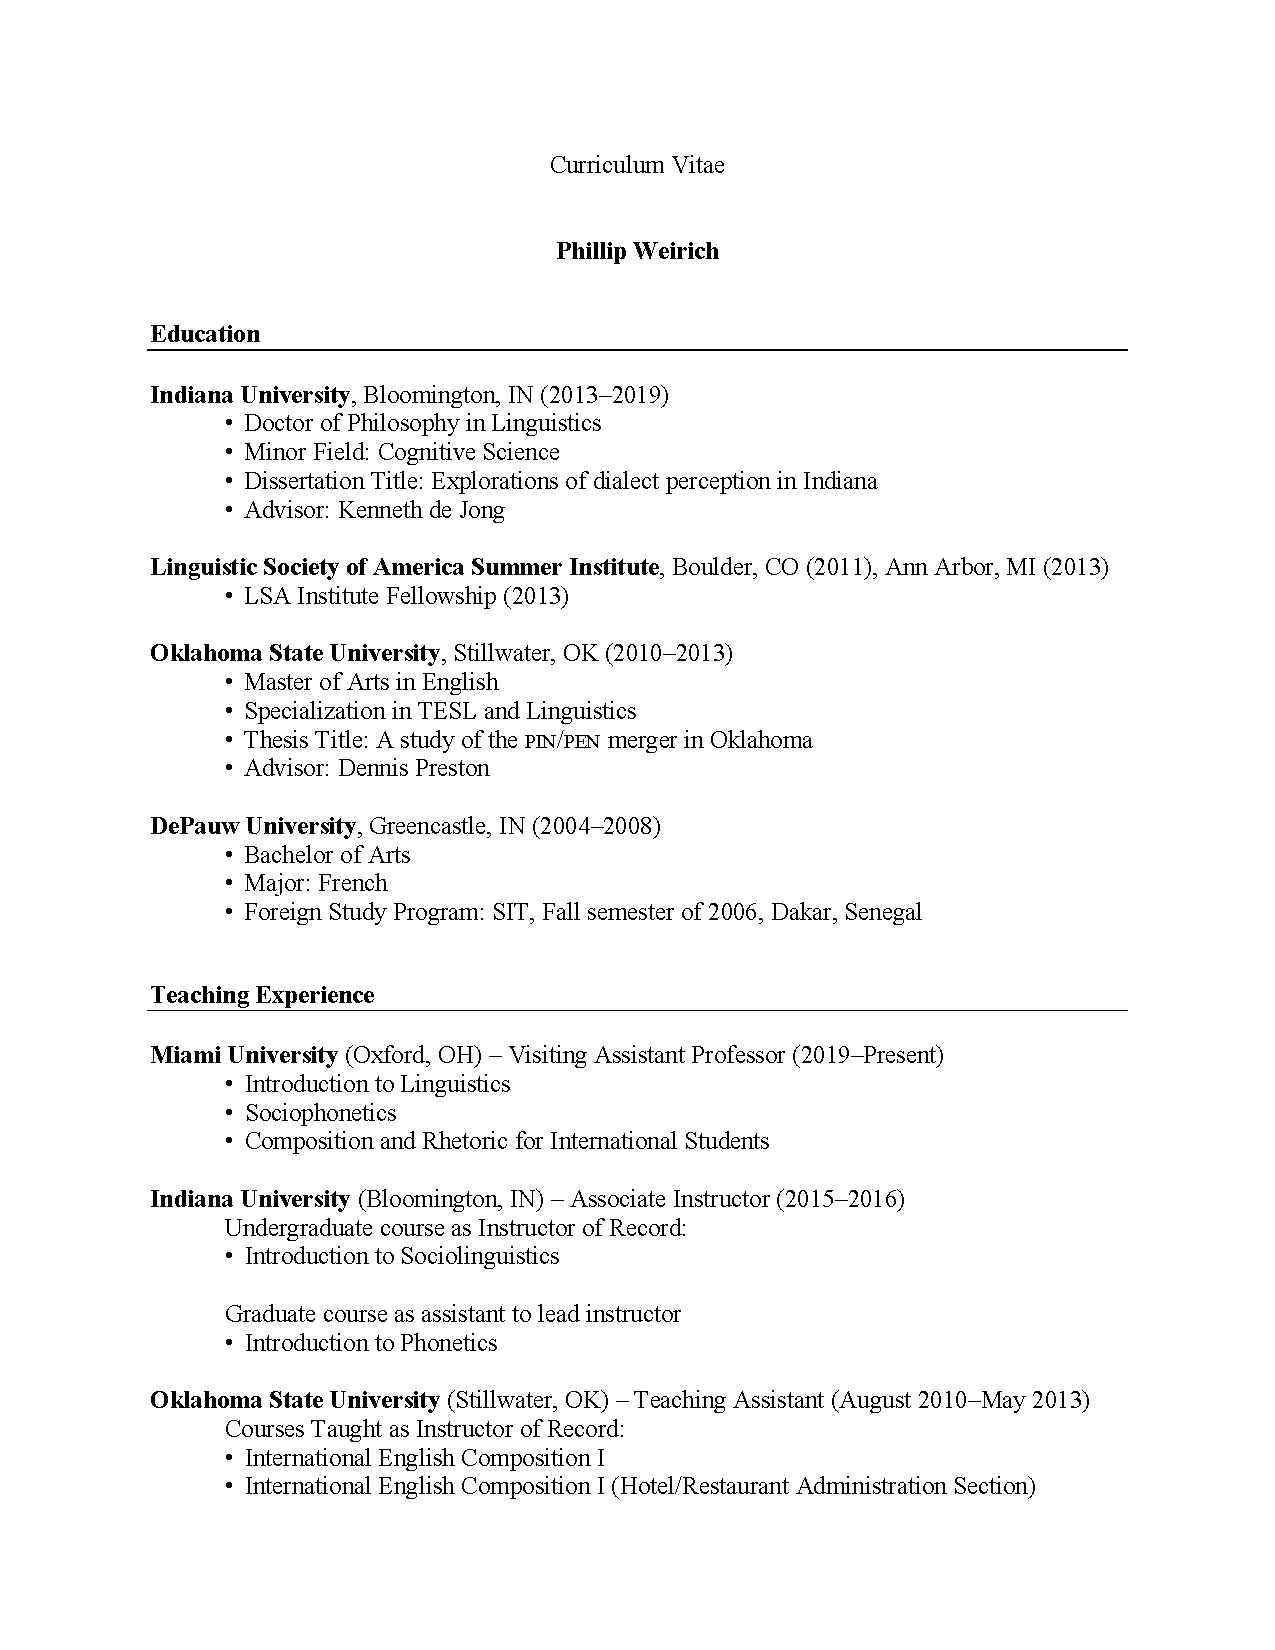
\includepdf[pages=-]{Weirich_CV_28_Sept_2019.pdf} 


\end{document}
